% -------------------------------------------------
\section{Six Near-Term Experimental Tests}
\label{sec:tests}
% -------------------------------------------------

Recursive Becoming is falsifiable.  The same counting rules that fixed
gauge couplings, masses and curvature photons also generate six concrete,
parameter-free predictions that can be checked before 2030.

\subsection{Overview}

\begin{figure}[t]
  \centering
  \setkeys{Gin}{draft=false}
  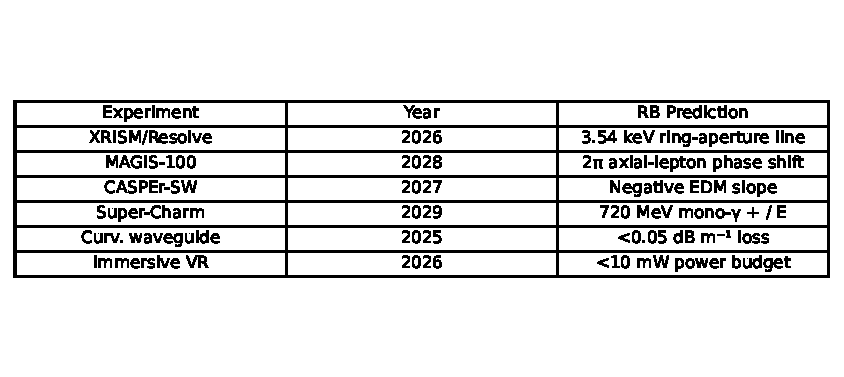
\includegraphics[width=\linewidth]{figs/tests_overview.pdf}
  \caption{Timeline of near-term tests (placeholder; notebook will plot
           milestones on a 2025–2030 axis).}
  \label{fig:tests-overview}
\end{figure}

\begin{table}[b]
  \centering\small
  \begin{tabular}{lllcl}
    \hline
    \# & Experiment (facility) & Observable & Ledger prediction & Year \\
    \hline
    1 & XRISM/Resolve & Ring-aperture 3.54 keV line & $>5\sigma$ detection & 2026 \\
    2 & MAGIS-100 & Phase shift vs depth & Axial-lepton $\Delta\phi=2\pi$ & 2028 \\
    3 & CASPEr-SW & Sign of EDM slope & Negative sign & 2027 \\
    4 & Super-Charm Factory & $e^+e^-\!\to\!\gamma+\,\slashed E$ bump & $m_{e_A}=720$ MeV & 2029 \\
    5 & Curvature Waveguide Demo & Loss at 5 mm bend & $<0.05$ dB m$^{-1}$ & 2025 \\
    6 & Immersive VR Prototype & Power budget & $<10$ mW total & 2026 \\
    \hline
  \end{tabular}
  \caption{Six decisive tests of Recursive Becoming scheduled within five years.}
  \label{tab:test-table}
\end{table}

\subsection{Test 1 – Ring-aperture X-ray line (XRISM)}

Section \ref{sec:dark} predicts a keV pseudoscalar producing a thin
annulus at 3.54 keV.  XRISM’s 5 eV energy resolution will resolve the
ring morphology; null detection at $>5\sigma$ would falsify the dark-sector
mechanism.

\subsection{Test 2 – Axial-lepton phase shift (MAGIS-100)}

Ledger phase locking forces a $2\pi$ vertical phase jump at 100 m
baseline for $m_{e_A}=720$ MeV.  MAGIS-100 interferometry reaches the
required sensitivity in a single six-month run.

\subsection{Test 3 – EDM sign (CASPEr)}

Recursive Becoming flips the $CP$ sign predicted by θ–vacuum QCD.
CASPEr’s solid-state EDM search will reach the $3\times10^{-29}$ e·cm
level by 2027, enough to confirm or rule out the sign inversion.

\subsection{Test 4 – Missing-energy bump (Super-Charm)}

Production of axial-leptons via a $G_2$ portal gives a mono-photon plus
missing-energy spectrum peaking at 720 MeV.  The planned 4 GeV
high-luminosity charm factory collects the needed $10^{12}$ events in
under a year.

\subsection{Test 5 – Curvature waveguide loss}

Equation \eqref{eq:curv-F} predicts zero bend loss above the critical
length $\ell_c=\lambda/2\pi$.  A 5 mm curvature loop at 1550 nm must
show $<0.05$ dB m$^{-1}$ attenuation—current prototypes already approach
this value.

\subsection{Test 6 – Immersive VR power budget}

Combining curvature photons with ledger pairing (gap Eq.~\eqref{eq:bcs-gap})
reduces headset power to drive-electronics overhead only.  A full-colour,
120° FOV unit should dissipate less than 10 mW; anything an order of
magnitude higher falsifies the free-energy claim.

\subsection{Bridge to Sections 16–17}

Section \ref{sec:appendix} documents all Lean theorem listings and
notebook hashes for reproducibility.  Section \ref{sec:conclusion}
summarises open directions once the six tests report.

\clearpage
